\documentclass{beamer}

\mode<presentation> {

% The Beamer class comes with a number of default slide themes
% which change the colors and layouts of slides. Below this is a list
% of all the themes, uncomment each in turn to see what they look like.

%\usetheme{default}
%\usetheme{AnnArbor}
%\usetheme{Antibes}
%\usetheme{Bergen}
%\usetheme{Berkeley}
%\usetheme{Berlin}
%\usetheme{Boadilla}
%\usetheme{CambridgeUS}
%\usetheme{Copenhagen}
%\usetheme{Darmstadt}
%\usetheme{Dresden}
%\usetheme{Frankfurt}
%\usetheme{Goettingen}
%\usetheme{Hannover}
%\usetheme{Ilmenau}
%\usetheme{JuanLesPins}
%\usetheme{Luebeck}
%\usetheme{Madrid}
%\usetheme{Malmoe}
%\usetheme{Marburg}
%\usetheme{Montpellier}
%\usetheme{PaloAlto}
\usetheme{Pittsburgh}
%\usetheme{Rochester}
%\usetheme{Singapore}
%\usetheme{Szeged}
%\usetheme{Warsaw}

% As well as themes, the Beamer class has a number of color themes
% for any slide theme. Uncomment each of these in turn to see how it
% changes the colors of your current slide theme.

%\usecolortheme{albatross}
%\usecolortheme{beaver}
%\usecolortheme{beetle}
%\usecolortheme{crane}
%\usecolortheme{dolphin}
%\usecolortheme{dove}
%\usecolortheme{fly}
%\usecolortheme{lily}
%\usecolortheme{orchid}
%\usecolortheme{rose}
%\usecolortheme{seagull}
%\usecolortheme{seahorse}
%\usecolortheme{whale}
%\usecolortheme{wolverine}

%\setbeamertemplate{footline} % To remove the footer line in all slides uncomment this line
%\setbeamertemplate{footline}[page number] % To replace the footer line in all slides with a simple slide count uncomment this line

%\setbeamertemplate{navigation symbols}{} % To remove the navigation symbols from the bottom of all slides uncomment this line
}

\usepackage{graphicx} % Allows including images
\usepackage{booktabs} % Allows the use of \toprule, \midrule and \bottomrule in tables
\usepackage{listings}
\usepackage{color}
\usepackage{float}


\definecolor{dkgreen}{rgb}{0,0.6,0}
\definecolor{gray}{rgb}{0.5,0.5,0.5}
\definecolor{mauve}{rgb}{0.58,0,0.82}

\lstset{
	frame=single,
	language=scala,
	belowskip=3mm,
	showstringspaces=false,
	columns=flexible,
	captionpos=b,
	basicstyle={\small\ttfamily},
	numbers=left,
	numbersep=5pt,
	%numbers=none,
	numberstyle=\tiny\color{gray},
	keywordstyle=\color{blue},
	commentstyle=\color{dkgreen},
	stringstyle=\color{mauve},
	breaklines=true,
	breakatwhitespace=true,
	tabsize=4
}
%----------------------------------------------------------------------------------------
%	TITLE PAGE
%----------------------------------------------------------------------------------------

\title[Short title]{Lightweight Distributed Service} % The short title appears at the bottom of every slide, the full title is only on the title page

\author{Yesheng Ma, Zucheng Wu, Yikai Zou} % Your name
\institute[SJTU] % Your institution as it will appear on the bottom of every slide, may be shorthand to save space
{
Shanghai Jiao Tong University
}
\date{\today} % Date, can be changed to a custom date

\begin{document}

\begin{frame}
\titlepage % Print the title page as the first slide
\end{frame}

\begin{frame}
\frametitle{Overview}
\tableofcontents % Throughout your presentation, if you choose to use \section{} and \subsection{} commands, these will automatically be printed on this slide as an overview of your presentation
\end{frame}

%----------------------------------------------------------------------------------------
%	PRESENTATION SLIDES
%----------------------------------------------------------------------------------------

%------------------------------------------------
\section{Introduction to distributed services} 

\begin{frame}{What are distributed services?}
Some examples are:

\begin{itemize}
\item Distributed key-value database.
\item Distributed lock service.
\item Replicated state machine(RSM).
\end{itemize}
\end{frame}

\begin{frame}{Why distributed services?}

\begin{itemize}
\item To make services highly available.
\item To make the system fault tolerant.
\item The system can recover after machine failure.
\end{itemize}

\end{frame}


\begin{frame}{How to build distributed services?}
\emph{\Large Consensus!} A system is available if the majority is alive.\\[1cm]

Early works date back to Leslie Lamport's 1989 paper on \emph{Paxos}.\\
But Paxos is famous for its difficulty to understand.\\[1cm]

\emph{Raft} comes to our rescue, which is easier to understand with an explicit leader.

\begin{figure}[H]
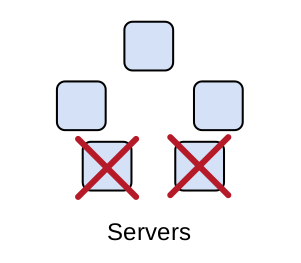
\includegraphics[width=2cm]{major.png}
\end{figure}

\end{frame}

\section{Raft Overview}


\begin{frame}
\frametitle{What is Raft}
Raft has two key components:
\begin{enumerate}
\item Leader election:
\begin{itemize}
\item A server is elected leader if most peers vote for it.
\item Only a server with an up-to-date log can become a leader.
\end{itemize}
\item Log replication:
\begin{itemize}
\item Clients send commands to leader.
\item Leader replicates its logs to other followers.
\end{itemize}
\end{enumerate}
\end{frame}


\section{Our Implementation}

\begin{frame}
\frametitle{Our Implementation: Overview}
Our goal:
\begin{itemize}
\item KISS: keep it simple, stupid, and easy to reason about.
\item Lightweight: about 4000 locs.
\item Cross platform.
\item Extensible.
\end{itemize}
\end{frame}


\begin{frame}
\frametitle{Our Implementation: Language}
Written with the Go programming language:
\begin{itemize}
\item A statically-typed PL with useful concurrent features.
\item Multiple platforms: from PC to Android devices.
\item Especially suitable to build network applications like Raft.
\end{itemize}
\end{frame}


\begin{frame}
\frametitle{Our Implementation: Network Simulation}
Real world network is not reliable.\\[1cm]

We simulates three kinds of RPC failures:
\begin{itemize}
\item Packet loss.
\item Long delays of packet transmission.
\item Reordering of packets.
\end{itemize}
\end{frame}

\begin{frame}
\frametitle{Our Implementation: Synchronization}
{\Large Say no to locks}! Only one mutex lock used.\\[1cm]

Instead use channels for synchronizations between threads:
\begin{enumerate}
\item The Raft entity receives timeouts/replies and redirects it to a respective channel.
\item A working thread takes the message from a channel and begins to work on it.
\item Once the working thread is done, send result back to the Raft entity.
\end{enumerate}
\end{frame}


\begin{frame}
\frametitle{Our Implementation: Performance}
Current version of our system can handle about 10 transactions per second.\\[1cm]

We have optimized the system to do batch log replication, i.e. replicate multiple log entries in a single remote procedure call.
\end{frame}


\begin{frame}
\frametitle{Future Work}
\begin{itemize}
\item Interface to real world network environment.
\item Network topology for scalability.
\item Network aware election timeout setting.
\end{itemize}
\end{frame}


\begin{frame}
\Huge{\centerline{Demo}}
\end{frame}

\begin{frame}
\Huge{\centerline{The End}}
\end{frame}

%----------------------------------------------------------------------------------------

\end{document} 